\section{Execution Time and Energy of the Selected Models}\label{sec:energy}

The cost $C_\rho$ in \eqref{eq:cost} counts the operations of the identified polynomial with a weight $\rho$ that must
reflect the platform; it does not by itself establish that cheaper structures run faster or consume less energy. This section reports historical measurements of free-run simulation over the validation data. Timing characterises the relation between operations and runtime; power integration estimates energy; carbon intensity converts energy to emissions. These measurements read stored models and do not alter the search objectives or its results. The corrected models require a new session, which has not yet been performed.

\subsection{Reconstruction and execution implementations}

For every run of SO, and of MO-lex and Green MGGP under both weights, the model $\mathcal M_\tau$ was rebuilt,
re-estimated on the identification data and simulated in free run over the validation input, which is the computation
behind the validation NRMSE of Table~\ref{tab:results}. The rebuilt models reproduced the stored cost and validation
error exactly for \enNModels{} of the \enNRecords{} runs; the remaining SO run on E3, whose validation simulation had
failed, is treated as missing. Each model was executed by two implementations whose outputs agreed to within
$\enMaxSimDiff$. The \emph{canonical} simulator is straight-line Python code generated from the duplicate-free
polynomial, so that each sample executes exactly the $a(\Rs)$ additions and $b(\Rs)$ multiplications counted by
$C_\rho$. The \emph{package} simulator is the free-run predictor of the \texttt{mggp} package, which
evaluates every gene, duplicates included, on windows of NumPy arrays; it represents the cost incurred by a user of the
package as distributed.\footnote{The package keeps only $n$ past outputs in its free-run window and delays them
circularly, so a factor $y(k-1-n)$ is read as $y(k-1)$; the canonical simulator uses the intended delays. Among the
selected models this affects only genes whose coefficients are below $10^{-15}$, hence the agreement of the two
outputs.}

\subsection{Timing and power measurement}
The execution time of each model was taken as the median of five batches of repeated simulations, each lasting at
least $50$~ms. Energy was measured on an Apple \enChip{} system-on-chip with Python~3.13 on mains power, from the
combined CPU, GPU and neural-engine power reported by \texttt{powermetrics} every $100$~ms. One measurement block
repeated complete cycles over the selected models of one example, configuration and simulator, so that every run
carried the same weight, for at least \enBlockS~s. Each of \enRounds{} rounds visited the \enNGroups{} groups in a
seeded random order and was bracketed by idle blocks of the same length, giving \enNBlocks{} blocks in about
\enDuration~min. The energy of one simulation is
\begin{equation}
E_\mathrm{sim}=\frac{E_\mathrm{block}-\tilde P_\mathrm{idle}\,t_\mathrm{block}}{n_\mathrm{sim}},
\label{eq:esim}
\end{equation}
where $\tilde P_\mathrm{idle}$ is the median power of all idle blocks, chosen before the measurement because it is
robust to an idle block disturbed by background activity. The idle power ranged from \enIdleMinW{} to
\enIdleMaxW~W, and subtracting instead the mean of the two idle blocks around each round changes the energy ratios
reported below by less than $0.05$ percentage points. The energy equation uses measured power and elapsed time, not the arithmetic objective. Carbon conversion is $\mathrm{CO_2e}=E_{\mathrm{sim}}\,I_{\mathrm{grid}}$, with energy expressed in kWh. Emissions follow from $E_\mathrm{sim}$ and the grid carbon
intensity of \enCountry{}, \enCI{}~gCO$_2$e/kWh, taken from the CodeCarbon energy-mix data~\cite{codecarbon}. CodeCarbon supplies the carbon-intensity factor only; energy is measured by \texttt{powermetrics}. Green
MGGP with $\rho=1$ is compared with SO, with MO-lex ($\rho=1$) and with Green MGGP under $\rho_K$ over the rounds, with
the tests of Section~\ref{sec:setup}, and energy ratios to SO are formed within each round.

\subsection{Time-based assessment of the declared weights}
Fig.~\ref{fig:exectime} relates the execution time per simulated sample to the structure of the \enNStruct{} distinct
canonical polynomials selected in all runs. For the canonical simulator, a least-squares fit of
$t=t_0+t_+\,a+t_\times b$ explains the times with $R^2=\enCanRtwoOps$, with $t_+=\enTadd$~ns per addition and
$t_\times=\enTmul$~ns per multiplication. These fitted coefficients include CPython execution and dispatch overhead and come from search-selected structures, rather than an independent arithmetic microbenchmark. They characterise this implementation on this laptop, not instruction-level hardware costs. The measured weight $t_\times/t_+=\enMulAdd$ is of order one, as was the
value of $0.98$ obtained in a pilot session with the models selected under $\rho_K$, and an order of magnitude below
$\rho_K\approx\rhoK$. Accordingly, the operation count $C_1$ predicts the time better ($R^2=\enCanRtwoOne$) than the
bit-level cost $C_{\rho_K}$ ($R^2=\enCanRtwoK$): on this interpreted binary64 implementation, the execution is
dominated by the dispatch of each operation rather than by the bit-level work of multiplication. The unit weight is
used rather than the fitted ratio because the latter reflects implementation details of the interpreter, such as the
indexing of delayed values, that differ between sessions and platforms.

\begin{figure}[t]
\centering
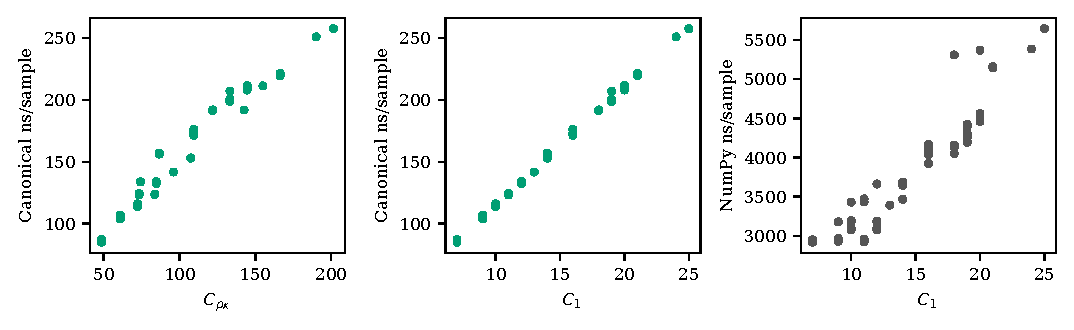
\includegraphics[width=\textwidth]{figures/fig_exec_time.pdf}
\caption{Execution time per simulated sample of the \enNStruct{} distinct canonical polynomials selected over all
runs and both weights, against the Karatsuba-weighted cost $C_{\rho_K}$ (a) and the operation count $C_1=a+b$ (b), with
least-squares lines; (c) the same models executed by the package free-run predictor (logarithmic scale).}
\label{fig:exectime}
\end{figure}

The package simulator is about \enOverhead{} times slower and its time is only weakly related to the cost (Spearman
correlation \enPkgRho{} with $C_1$, $R^2=\enPkgRtwoOne$). It evaluates every gene of the individual, including
duplicates and genes with negligible coefficients, through array operations whose overhead does not depend on the
degree, so its time is governed by the number and size of the gene trees rather than by the executed structure.

\subsection{Energy and emissions}
The net power drawn during simulation was nearly constant, about \enNetWCan~W for the canonical simulator and between
\enNetWPkgLo{} and \enNetWPkgHi~W for the package simulator, so the energy of a simulation follows its execution
time. Table~\ref{tab:energy} and Fig.~\ref{fig:energy} summarise the measurements. With the canonical simulator, the
models selected by Green MGGP required less energy than the SO models on every example, with median per-round ratios
of \EBCanGreenEratio, \ECCanGreenEratio{} and \EDCanGreenEratio{} and complete separation of the rounds
($A_{12}=0.00$). They also required less energy than the MO-lex models on E2 and E3, whereas on E1 both methods select
the same nine-operation structures and their energies do not differ significantly. The reductions follow the operation
counts of Table~\ref{tab:results} closely: on E3, for instance, the median counts of $14$ and $20.5$ operations per
sample are in the ratio $0.68$, and the measured energy ratio is \EDCanGreenEratio.

\begin{figure}[!htb]
\centering
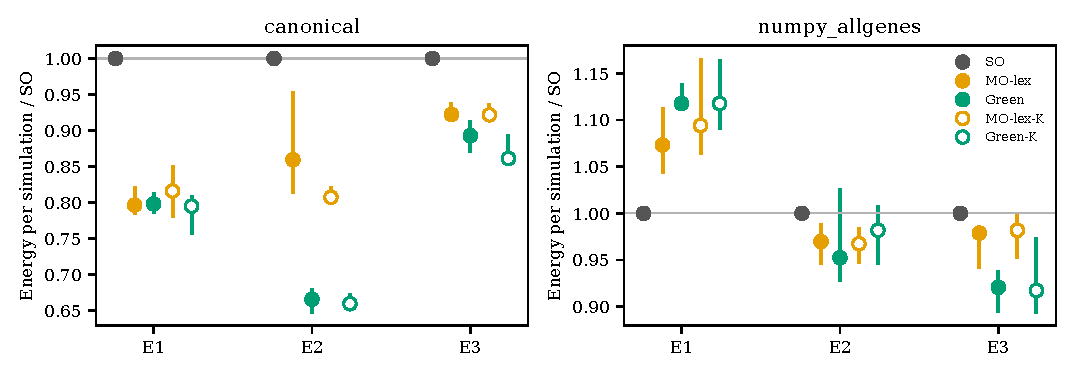
\includegraphics[width=\textwidth]{figures/fig_energy.pdf}
\caption{Energy per free-run simulation of the selected models relative to SO, formed within each of the
\enRounds{} measurement rounds: median (markers) and interquartile range (bars) over the rounds, for the canonical (a)
and package (b) simulators. Filled markers: $\rho=1$; open markers: $\rho_K$. The absolute SO energies are given on the
right.}
\label{fig:energy}
\end{figure}

\begin{table}[!htbp]
\centering
\caption{Execution of the corrected selected models: median time, net energy and estimated carbon per simulation over ten measurement rounds. Canonical execution evaluates distinct monomials; all-gene NumPy execution uses corrected delays. Suffix K denotes searches under $\rho_K$.}
\label{tab:corrected_energy}
\setlength{\tabcolsep}{3pt}
\begin{tabular}{llrrrrrr}
\toprule
 & & \multicolumn{3}{c}{Canonical polynomial} & \multicolumn{3}{c}{All-gene NumPy} \\
\cmidrule(lr){3-5}\cmidrule(lr){6-8}
Ex. & Method & Time ($\mu$s) & Energy ($\mu$J) & CO$_2$e ($\mu$g) & Time ($\mu$s) & Energy ($\mu$J) & CO$_2$e ($\mu$g) \\
\midrule
E1 & SO & 9.91 & 65.4 & 0.00528 & 313 & 2.11e+03 & 0.17 \\
E1 & MO-lex & 7.78 & 51.6 & 0.00417 & 329 & 2.31e+03 & 0.186 \\
E1 & Green & 7.79 & 52.2 & 0.00422 & 337 & 2.37e+03 & 0.192 \\
E1 & MO-lex-K & 7.82 & 52.5 & 0.00424 & 334 & 2.32e+03 & 0.187 \\
E1 & Green-K & 7.78 & 51.1 & 0.00413 & 330 & 2.35e+03 & 0.19 \\
\midrule
E2 & SO & 11.7 & 76.7 & 0.0062 & 338 & 2.34e+03 & 0.189 \\
E2 & MO-lex & 9.49 & 65.7 & 0.0053 & 328 & 2.24e+03 & 0.181 \\
E2 & Green & 7.66 & 51.2 & 0.00414 & 324 & 2.23e+03 & 0.18 \\
E2 & MO-lex-K & 9.44 & 62.7 & 0.00507 & 326 & 2.23e+03 & 0.18 \\
E2 & Green-K & 7.65 & 50.4 & 0.00407 & 321 & 2.25e+03 & 0.182 \\
\midrule
E3 & SO & 38.4 & 251 & 0.0203 & 848 & 5.8e+03 & 0.469 \\
E3 & MO-lex & 35.3 & 232 & 0.0188 & 832 & 5.55e+03 & 0.448 \\
E3 & Green & 33.6 & 228 & 0.0184 & 789 & 5.26e+03 & 0.425 \\
E3 & MO-lex-K & 35.4 & 233 & 0.0188 & 830 & 5.6e+03 & 0.452 \\
E3 & Green-K & 32.9 & 219 & 0.0177 & 783 & 5.38e+03 & 0.434 \\
\bottomrule
\end{tabular}
\end{table}




The weight used during identification matters where it changes the selected structures. On E1 and E2, where the two
weights mostly select the same or equally long models, Green MGGP with $\rho=1$ and with $\rho_K$ consume the same
energy with the canonical simulator. On E3, the models selected with $\rho=1$ need $2\%$ less energy than those
selected with $\rho_K$ with the canonical simulator and $8\%$ less with the package simulator, both significant, so the
unit-weight scenario yields structures that are also cheaper to execute in this historical session.

With the package simulator, the advantage over SO is smaller but significant on every example, with ratios of
\EBPkgGreenEratio, \ECPkgGreenEratio{} and \EDPkgGreenEratio, and over MO-lex on E2 and E3. Expressed per $10^6$
simulations of the validation record, the E3 models selected by Green MGGP correspond to \EDCanGreenCO~mg CO$_2$e
with the canonical simulator, against \EDCanSOCO~mg for SO, and to \EDPkgGreenCO~g against \EDPkgSOCO~g with the package
simulator. The implementation thus matters more than the structure: the same models differ by two orders of magnitude
between the two simulators, and the benefit of a cheaper
structure is realised in full only when the canonical polynomial is executed.

These measurements concern interpreted code on one laptop system-on-chip in one session, not the embedded processors
on which identified models are often deployed and where multiplications may cost more. They show that the ordering
induced by $C_\rho$ carries over to measured time and energy for canonical execution, and that $\rho$ should be
calibrated on the target platform before identification.

\FloatBarrier
